%\ccChapterSubTitle{\alphashapeRevision, \alphashapeDate}
\begin{ccTexOnly}
%\vspace*{-1cm}
\begin{center}
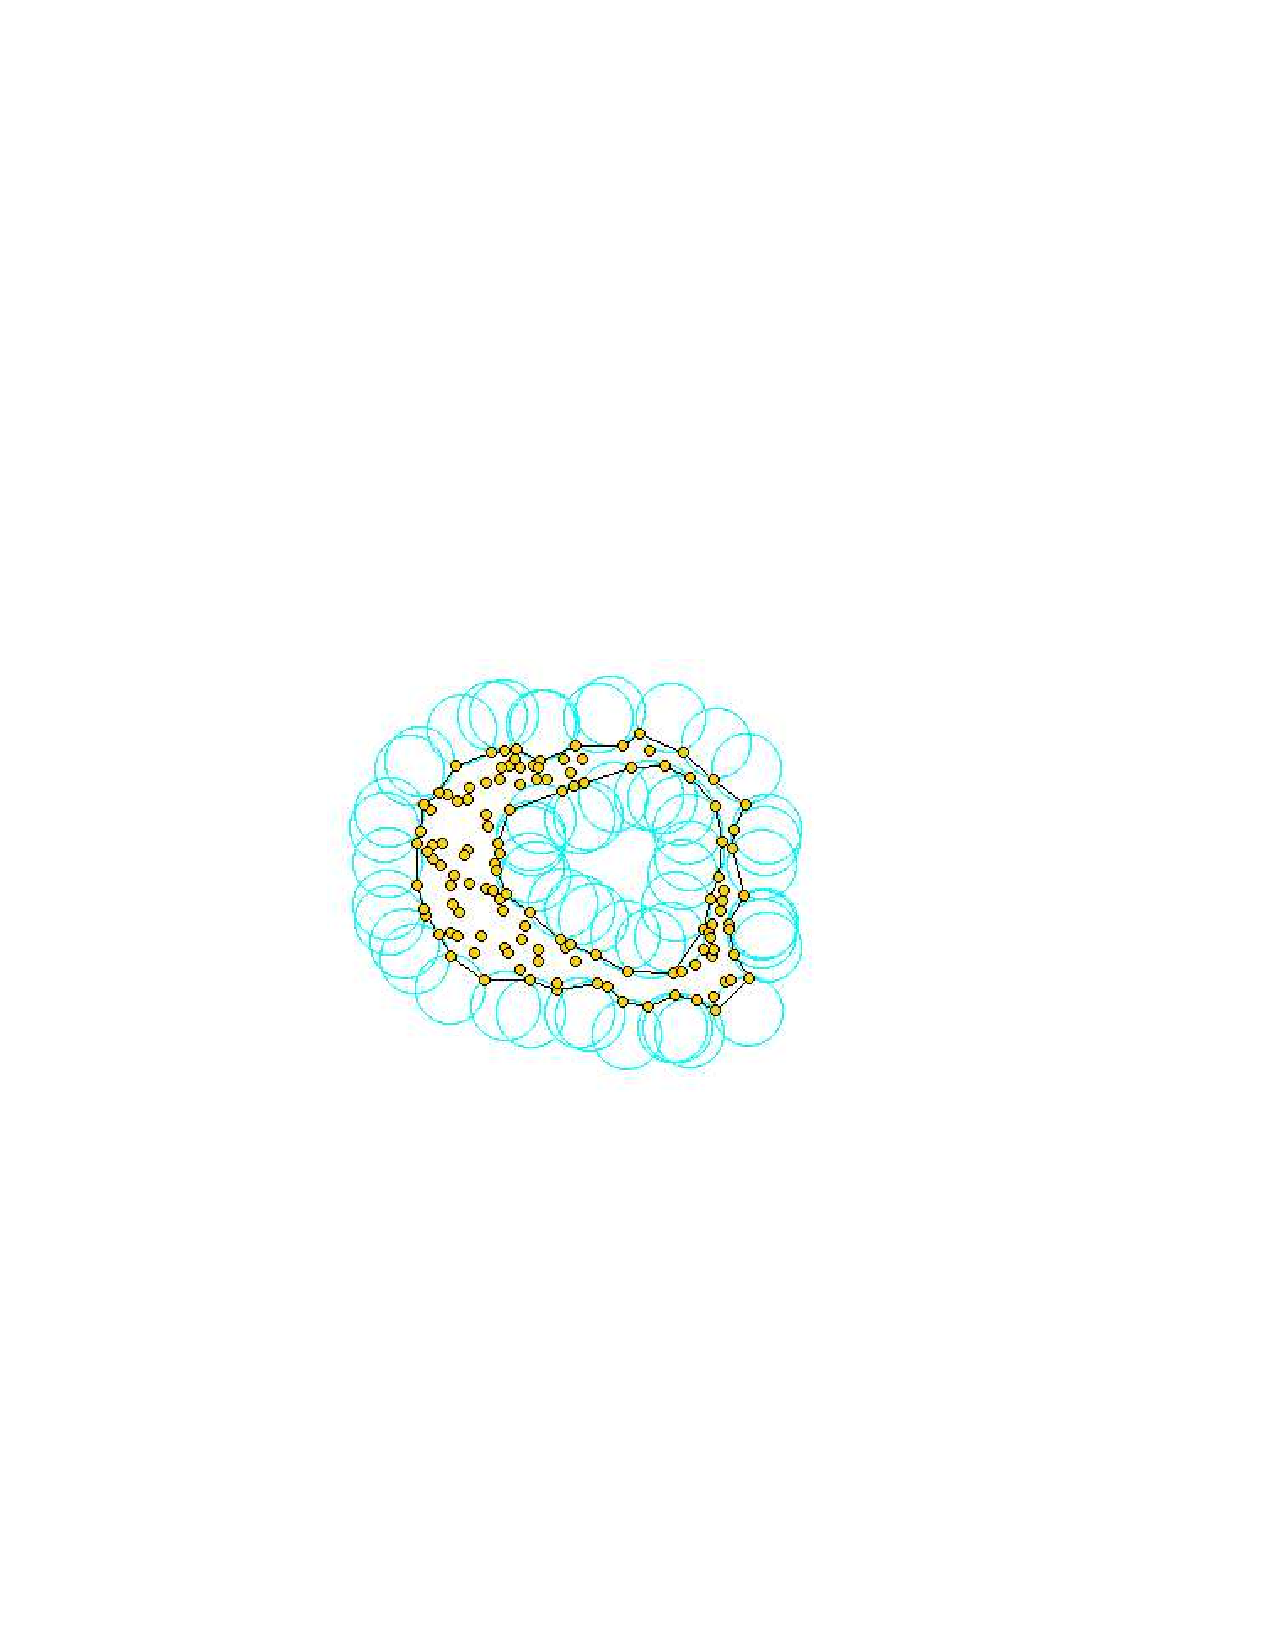
\includegraphics{Alpha_shapes_3/alphashape} 
\end{center}
\end{ccTexOnly}
\begin{ccHtmlOnly}
<img border=0 src="./alphashape.gif"  align=center  alt="alphashape">
\end{ccHtmlOnly}

Assume we are given a set $S$ of points in 2D or 3D and we'd like to
have something like ``the shape formed by these points.'' This is
quite a vague notion and there are probably many possible
interpretations, the alpha shape  being one of them. Alpha shapes
can be used for shape reconstruction from a dense unorganized set of
data points. Indeed, an alpha shape  is demarcated by a frontier,
which is a linear approximation of the original shape \cite{bb-srmua-97t}.

As mentionned in Edelsbrunner's and M\"ucke's paper \cite{em-tdas-94},
one can intuitively think of an alpha shape  as the
following. Imagine a huge mass of ice-cream making up the space $\R^3$
and containing the points as ``hard'' chocolate pieces. Using one of
those sphere-formed ice-cream spoons we carve out all parts of the
ice-cream block we can reach without bumping into chocolate pieces,
thereby even carving out holes in the inside (eg. parts not reachable
by simply moving the spoon from the outside). We will eventually end
up with a (not necessarily convex) object bounded by caps, arcs and
points. If we now straighten all ``round'' faces to triangles and line
segments, we have an intuitive description of what is called the
alpha shape  of $S$. Here's an example for this process in 2D (where
our ice-cream spoon is simply a circle):

Alpha shapes depend on a parameter $\alpha$ from which they
are named.                                                                  
What is $\alpha$ in the ice-cream game?  $\alpha$ is the squared radius of the
carving spoon. A very small value will allow us to eat up all of the
ice-cream except the chocolate points themselves. Thus we already see
that the alpha shape  degenerates to the point-set $S$ for
$\alpha \rightarrow 0$. On the other hand, a huge value of $\alpha$
will prevent us even from moving the spoon between two points since
it's way too large. So we will never spoon up ice-cream lying in the
inside of the convex hull of $S$, and hence the alpha shape  for
$\alpha \rightarrow \infty$ is the convex hull of $S$.\footnote{ice cream, ice cream!!!
The wording of this introductory paragraphs is borrowed from  Kaspar Fischer's
`` Introduction to Alpha Shapes'' which can be found at 
http://n.ethz.ch/student/fischerk/alphashapes/as/index.html.
The picture has been taken from Walter Luh's homepage at
http://www.stanford.edu/\~wluh/cs448b/alphashapes.html.}


\section{Definitions}

% Alpha shapes are the generalization of the convex hull of a point
% set. Let $S$ be a finite set of points in $\R^d$, $d = 2,3$ and
% $\alpha$ a parameter with $0 \leq \alpha \leq
% \infty$. For $\alpha = \infty$, the alpha shape  is the convex hull of $S$. As 
% $\alpha$ decreases, the alpha shape  shrinks and develops cavities,
% as soon as a sphere of radius $\sqrt{\alpha}$ can be put inside.
% Finally, for $\alpha = 0$, the alpha shape  is the set $S$ itself.

More precisely, the definition of alpha shapes is based on an underlying
triangulation that may be a Delaunay triangulation 
in case of basic alpha shapes 
or a regular triangulation 
(cf. \ref{Triangulation3-sec-class-Regulartriangulation})
in case of weighted alpha shapes.

Let us consider the basic case with a Delaunay triangulation.
We first define the alpha complex  of the set of points $S$. 
The  alpha complex is a subcomplex 
of the Delaunay triangulation.
For a given value of $\alpha$, the alpha complex includes
all the simplices in the Delaunay triangulation which have
an empty  circumsphere with squared radius equal or smaller than $\alpha$.
Here ``empty'' means  that the open sphere 
do not include  any points of $S$.
The alpha shape is then simply the domain covered by the simplices
of the alpha complex (see \cite{em-tdas-94}).

In general, an alpha complex is a non-connected and non-pure complex.
This means in particular that the alpha complex may have
singular faces.  For $0 \leq k \leq d-1$,
a $k$-simplex of the alpha complex  is said to be
singular if it is not a facet of a $(k+1)$-simplex of the complex
CGAL provides two versions of the alpha shapes. In the general mode,
the alpha shapes correspond strictly to the above definition.
The regularized mode provides a regularized version of the alpha shapes
corresponding to the domain covered by a regularized version
of the alpha complex where singular faces are removed.





% The {\em basic alpha shapes} (cf. \ref{I1_SectClassicAS2D}) associated
% with the Delaunay triangulations (cf. \ref{I1_Sect_Delaunay}), in the
% other hand, the {\em weighted alpha shapes}
% (cf. \ref{I1_SectWeightedAS2D}) associated with the regular
% triangulations (cf. \ref{I1_Sect_Regular}).

The alpha shapes of a  set of points 
$S$ form a discrete family, even though they
are defined for all real numbers $\alpha$.
The entire family of alpha shapes can be represented 
through  the underlying triangulation of $S$. In this representation
each $k$-simplex of the underlying triangulation is associated with an
interval that specifies for which values of $\alpha$ the $k$-simplex
belongs to the alpha complex. Relying on this fact, the family of
 alpha shapes can be computed efficiently and relatively
easily. Furthermore, we can select the optimal value
of  $\alpha$ to get an alpha shape including all data points
and having   less than a given number of connected components.
Also, the alpha-values allows to define a filtration on the
faces of the triangulation of a set of points. 
In this filtration, the faces of the triangulation are output
in increasing order of the alpha value  
for which they appear 
in the alpha complex.  In case of equal alpha value
lower dimensional faces are output first.



The definition is analog in the case of weigthed alpha shapes.
The input set is now a set of weighted points (which can be regarded
as spheres) and the underlying triangulation 
is the regular triangulation of this set.
Two spheres, or two weighted points , with centers $C_1, C_2$
and  radii $r_1, r_2 $ are said to be orthogonal iff 
$ C_1C_2 ^2 = r_1^2 + r_2^2$ and suborthogonal
iff  $ C_1C_2 ^2 < r_1^2 + r_2^2$.
For a given value of $\alpha$
the weighted alpha complex is formed with the simplices of the 
regular triangulation triangulation
such that there is a sphere orthogonal to the weighted points associated
with the vertices of the simplex  and suborthogonal to all the other
input weighted points. Once again the alpha shape is then defined as
the domain covered by a the alpha complex and arise in two versions
general or regularized.




%----------------------------------------------------------------------

\section{Functionality \label{I1_SectAlpha_Shape_3}}

The class \ccc{CGAL::Alpha_shape_3<Dt>} represents the whole
family of alpha shapes for a given set of points.
The class includes  the underlying triangulation \ccc{Dt}
of the set,  and associates to each $k$-face of this triangulation
 an interval specifying 
for which values of $\alpha$ the face belongs to the
alpha complex. 


The class \ccc{CGAL::Alpha_shape_3<Dt>} provides functions to set and
get the current $\alpha$-value, as well as an iterator that enumerates
the $\alpha$ values where the alpha shape changes.

The class provides member functions to classify for a given value
of $alpha$ the different faces of the triangulation as
\ccc{EXTERIOR}, \ccc{SINGULAR}, \ccc{REGULAR} or 
\ccc{INTERIOR} with respect
to the alpha shape. A $k$ face  on the boundary of the alpha complex
is said to be \ccc{REGULAR}  if it is a subface of the alpha complex
which is  a subface of some $k+1$ face of the alpha complex
and \ccc{SINGULAR} otherwise.

The class  provides also output iterators  to  get for a given $alpha$ value
the vertices, edges, facets and cells of the different types
(\ccc{EXTERIOR}, \ccc{SINGULAR}, \ccc{REGULAR} or 
\ccc{INTERIOR}).

Also the class has a filtration member function that, given
an  output iterator with \ccc{CGAL::object}
as value  type, outputs the faces of the triangulation 
according to the 
order of apparition in the alpha complex when alpha increases.
  

Finally, it provides a function to determine 
the smallest value $\alpha$
such that the alpha shape   satisfies the following two properties~\\
(ii) all data points are either on the boundary or in the interior 
   of the regularized version of the alpha shape  (no singular faces). \\
(i) The number of components is equal or less  than a given  number .

\smallskip
The current implementation is static, that is after its construction
points cannot be inserted or removed.
%----------------------------------------------------------------------

\section{Concepts and Models\label{I1_SectDtClass3D}}


We currently do not specify concepts for the underlying triangulation
type. Models that work for a basic alpha-shape are the classes
\ccc{CGAL::Delaunay_triangulation_3} and 
\ccc{CGAL::Triangulation_hierarchy_3} templatized with a Delaunay
triangulation. A model that works for a weighted alpha-shape is 
the class \ccc{CGAL::Regular_triangulation_3}.

The triangulation needs a geometric traits class as argument.
The requirements of this class are described in the 
concept \ccc{CGAL::AlphaShapeTraits_3} for which
the \cgal\ kernels are models in the non-weighted case, and for which
the class \ccc{CGAL::Weighted_alpha_shape_euclidean_traits_3} is model
in the weighted case.

The triangulation data structure of the triangulation with any 
has to be a model of the concept \ccc{CGAL::TriangulationDataStructure_3}.
However it must be parameterized with 
vertex and cell classes, which are model of the concepts
\ccc{AlphaShapeVertex_3} and \ccc{AlphaShapeCell_3}.
The package provides
by default the classes \ccc{CGAL::Alpha_shape_vertex_base_3<Gt>} 
and \ccc{CGAL::Alpha_shape_cell_base_3<Gt>}.




%----------------------------------------------------------------------

\section{Examples}
\subsection{Example for Basic Alpha-Shapes\label{I1_SectClassicAS3D}}

This example builds a basic alpha shape using a  Delaunay triangulation
as underlying triangulation.


\ccIncludeExampleCode{Alpha_shapes_3/alpha_shapes_3.C}


\subsection{Building Basic Alpha Shapes for Many Points}
When many points are input in the alpha shape, say more than 10 000,
it pays off to use a triangulation hierarchy as underlying triangulation
(cf. \ref{T3-concept-hierarchy}).

\ccIncludeExampleCode{Alpha_shapes_3/alpha_shapes_with_hierarchy_3.C}
%----------------------------------------------------------------------

\subsection{Example for Weighted Alpha-Shapes\label{I1_SectWeightedAS3D}}

The following examples build a weighted alpha shape requiring a
regular triangulation as underlying triangulation.
The alpha shape is build in \ccc{GENERAL} mode.


\ccIncludeExampleCode{Alpha_shapes_3/weighted_alpha_shapes_3.C}
